Configurar como principales los enlaces marcados:
  \begin{figure}[h]
    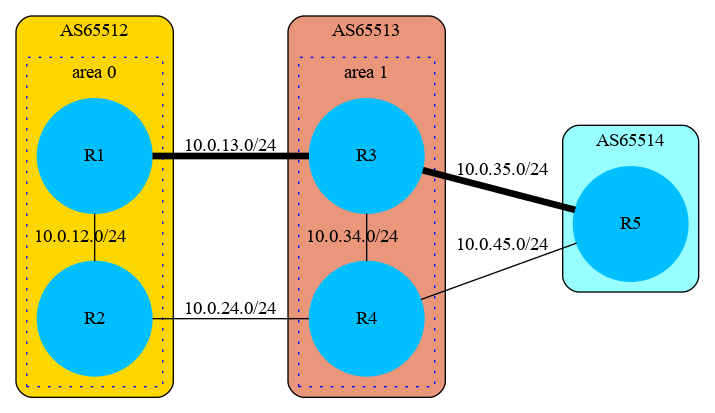
\includegraphics[width=12cm]{bgp_next_hop.png}
  \end{figure}

  Detalles a tener en cuenta:

  \begin{itemize}
    \item Las interfaces entre los nodos R1 - R3 y R2 - R4 han de ser pasivas
    \item La comunicación entre routeres del mismo AS es mediante iBGP/OSPF
    \item La comunicación entre los AS es mediante eBGP
    \item En el AS 65514 la comunicación con el router R5 es exclusivamente BGP
    \item Anuncios BGP explícitos:
    \begin{itemize}
      \item AS 65512: 172.12.0.0/16
      \item AS 65513: 172.13.0.0/16
      \item AS 65514: 172.14.0.0/16
    \end{itemize}
  \end{itemize}

  \begin{minted}{bash}
    # net.conf
    defsw br12 uml1.0 uml2.0
    defsw br13 uml1.1 uml3.0
    defsw br24 uml2.1 uml4.0
    defsw br34 uml3.1 uml4.1
    defsw br45 uml4.2 uml5.0
    defsw br35 uml3.2 uml5.1
  \end{minted}

  \begin{minted}{bash}
  # En cuanto se inician las UML1-4, editar el fichero /etc/quagga/daemons la línea
  bgpd=no
  ospfd=no
  # Por
  bgpd=yes
  ospfd=yes
  # Para UML5, solo cambiar el demonio bgpd=no por bgpd=yes
  # A continuación restart del servicio para todas las UML
  systemctl restart quagga
  # Verificar que se ospfd está corriendo
  systemctl status quagga
\end{minted}

  \begin{minted}{lexer.py:IOSLexer -x}
    ! UML1 (zebra.conf)
    conf[igure] term[inal]
    int[erface] eth0
    ip address 10.0.12.1/24
    no shutdown
    quit
    int[erface] eth1
    ip address 10.0.13.1/24
    no shutdown
    quit
    ip forwarding
    exit
    write
  \end{minted}

  \begin{minted}{lexer.py:IOSLexer -x}
    ! UML2 (zebra.conf)
    conf[igure] term[inal]
    int[erface] eth0
    ip address 10.0.12.2/24
    no shutdown
    quit
    int[erface] eth1
    ip address 10.0.24.1/24
    no shutdown
    quit
    ip forwarding
    exit
    write
  \end{minted}

  \begin{minted}{lexer.py:IOSLexer -x}
    ! UML3 (zebra.conf)
    conf[igure] term[inal]
    int[erface] eth0
    ip address 10.0.13.1/24
    no shutdown
    quit
    int[erface] eth1
    ip address 10.0.34.1/24
    no shutdown
    int[erface] eth2
    ip address 10.0.35.1/24
    no shutdown
    quit
    ip forwarding
    exit
    write
  \end{minted}

  \begin{minted}{lexer.py:IOSLexer -x}
    ! UML4 (zebra.conf)
    conf[igure] term[inal]
    int[erface] eth0
    ip address 10.0.24.2/24
    no shutdown
    quit
    int[erface] eth1
    ip address 10.0.34.2/24
    no shutdown
    int[erface] eth2
    ip address 10.0.45.1/24
    no shutdown
    quit
    ip forwarding
    exit
    write
  \end{minted}

  \begin{minted}{lexer.py:IOSLexer -x}
    ! UML5 (zebra.conf)
    conf[igure] term[inal]
    int[erface] eth0
    ip address 10.0.45.2/24
    no shutdown
    quit
    int[erface] eth1
    ip address 10.0.35.2/24
    no shutdown
    quit
    ip forwarding
    exit
    write
  \end{minted}

  \begin{minted}{lexer.py:IOSLexer -x}
    ! UML1 (ospf.conf)
    conf[igure] term[inal]
    router ospf
    ospf router-id 0.0.0.1
    network 10.0.12.0/24 area 0
    network 10.0.13.0/24 area 0
    p[assive-interface] eth1 ! El interfaz que comunica con el AS65513
    end
    write
  \end{minted}

  \begin{minted}{lexer.py:IOSLexer -x}
    ! UML2 (ospf.conf)
    conf[igure] term[inal]
    router ospf
    ospf router-id 0.0.0.2
    network 10.0.12.0/24 area 0
    network 10.0.24.0/24 area 0
    p[assive-interface] eth1 ! El interfaz que comunica con el AS65513
    end
    write
  \end{minted}

  \begin{minted}{lexer.py:IOSLexer -x}
    ! UML3 (ospf.conf)
    conf[igure] term[inal]
    router ospf
    ospf router-id 0.0.0.3
    network 10.0.13.0/24 area 1
    network 10.0.34.0/24 area 1
    network 10.0.35.0/24 area 1
    p[assive-interface] eth0 ! El interfaz que comunica con el AS65512
    end
    write
  \end{minted}

  \begin{minted}{lexer.py:IOSLexer -x}
    ! UML4 (ospf.conf)
    conf[igure] term[inal]
    router ospf
    ospf router-id 0.0.0.4
    network 10.0.24.0/24 area 1
    network 10.0.34.0/24 area 1
    network 10.0.35.0/24 area 1
    p[assive-interface] eth0 ! El interfaz que comunica con el AS65512
    end
    write
  \end{minted}

  \begin{minted}{lexer.py:IOSLexer -x}
    ! UML1 (bgp.conf)
    con[figure] t[erminal]
    router bgp 65512
    nei[ghbor] 10.0.13.2 remote-as 65513
    nei[ghbor] 10.0.12.2 remote-as 65512
    network 172.12.0.0/16
    nei[ghbor] 10.0.13.2 route-m[ap] FILTRO in
    route-map FILTRO permit 10
      se[t] l[ocal-preference] 200
    do write
  \end{minted}

  \begin{minted}{lexer.py:IOSLexer -x}
    ! UML2 (bgp.conf)
    con[figure] t[erminal]
    router bgp 65512
    nei[ghbor] 10.0.24.2 remote-as 65513
    nei[ghbor] 10.0.12.1 remote-as 65512
    do write
  \end{minted}

  \begin{minted}{lexer.py:IOSLexer -x}
    ! UML3 (bgp.conf)
    con[figure] t[erminal]
    router bgp 65513
    nei[ghbor] 10.0.13.1 remote-as 65512
    nei[ghbor] 10.0.35.2 remote-as 65514
    nei[ghbor] 10.0.34.2 remote-as 65513
    network 172.13.0.0/16
    nei[ghbor] 10.0.35.2 route-m[ap] FILTRO in
    route-map FILTRO permit 10
      se[t] l[ocal-preference] 200
    do write
  \end{minted}

  \begin{minted}{lexer.py:IOSLexer -x}
    ! UML4 (bgp.conf)
    con[figure] t[erminal]
    router bgp 65513
    nei[ghbor] 10.0.24.1 remote-as 65512
    nei[ghbor] 10.0.45.2 remote-as 65514
    nei[ghbor] 10.0.34.1 remote-as 65513
    do write
  \end{minted}

  \begin{minted}{lexer.py:IOSLexer -x}
    ! UML5 (bgp.conf)
    con[figure] t[erminal]
    router bgp 65514
    nei[ghbor] 10.0.35.1 remote-as 65513
    nei[ghbor] 10.0.45.1 remote-as 65513
    network 172.14.0.0/16
    do write
  \end{minted}

  Pruebas:
  \begin{minted}{lexer.py:IOSLexer -x}
    ! En una UML
    clear bgp * ! se borra toda la información BGP de las tablas de todos los routeres
    ! En cada uno de los nodos
    sh[ow] ip bgp
  \end{minted}

  \begin{itemize}
    \item Probar a cambiar el router que anuncia la network para comprobar
    que las rutas BGP son acordes a las políticas aplicadas
  \end{itemize}